\documentclass[../../main.tex]{subfiles}

\begin{document}
\section{Tree Tensor Networks}
    Now, we want to analyze the properties of these binary tree tensor networks further. It may not bother us how we construct increasingly bigger models that satisfy the bulk marginal property, we know that the model space of binary tree tensor networks is capable of producing a family of networks that satisfy this property.

    Furthermore, we may also constrain every tensor network to be non-negative and normalized. Of course, such networks are always constructable as well. We also allow for negative entries in the tensors. We also don't apply any function $f$ to the tensor output, the network outputs directly correspond to probabilities.

    One question we might ask is whether such a model space restricts the space of possible probability distributions, and if so by how much. As it turns out, in the most general case when allowing very large tensors in the networks, we can model \emph{any} probability distribution:

    \begin{proposition}
        Given any probability distribution $p: \Sigma^{2^k} \mapsto [0,1]$, we can always construct a binary tree tensor network $\mathcal{T}$ over $\Sigma^{2^k}$ s.t. $p \equiv S_{2^k, \mathcal{T}}$ (, where $\mathcal{T}$ has the properties like discussed above and has no constrains on the tensor sizes).
    \end{proposition}
    \vspace{-2.5em}
    \begin{proof}
        For clarity reasons, we only show how to construct $\mathcal{T}$ for $n = 2^k = 4$. The procedure can easily be extended to the general case.

        Our model structure is depicted in figure~\ref{fig:binary_tree_tensor_network_n_equals_four}.

        \begin{figure}[h]
        \centering
        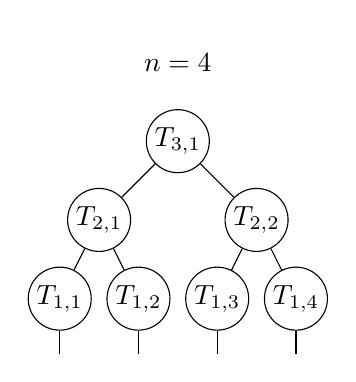
\begin{tikzpicture}[
            every node/.style={circle, draw, minimum size=8mm, inner sep=0pt},
            level distance=10mm,
            sibling distance=10mm,
            edge from parent/.style={draw},
            level 1/.style={sibling distance=20mm},
            level 2/.style={sibling distance=10mm}
        ]

        % Tree with 4 leaves
        \node[draw=none] at (1,0) {$n=4$};
        \node (t31) at (1, -1) {$T_{3,1}$} [grow=down]
        child {node (t21a) {$T_{2,1}$}
            child {node (t11c) {$T_{1,1}$}}
            child {node (t13) {$T_{1,2}$}}}
        child {node (t22) {$T_{2,2}$}
            child {node (t14) {$T_{1,3}$}}
            child {node (t15) {$T_{1,4}$}}};
        \draw (t11c) -- ++(0,-0.7);
        \draw (t13) -- ++(0,-0.7);
        \draw (t14) -- ++(0,-0.7);
        \draw (t15) -- ++(0,-0.7);

        \end{tikzpicture}
        \caption{Model structure of binary tree tensor networks for $n = 2^k = 4$.}
        \label{fig:binary_tree_tensor_network_n_equals_four}
    \end{figure}

    Now, we initialize the leaf matrices as identity matrices $\delta_2 \in \mathbb{R}^{|\Sigma| \times |\Sigma|}$. Thus, when contracting a leaf tensor with a one-hot encoded input vector at position $i$, we get the vector $v_j = \bm{1}[X_i = c_j], c_j \in \Sigma$.

    Now, the tensors in layer two are of the following form:
    \[
    T_{2, j}: |\Sigma| \times |\Sigma| \mapsto \mathbb{R}^{|\Sigma|^2} \quad .
    \]
    The outgoing axis may be index by $(X'_i, X'_{i + 1}) \in \Sigma^2$. The map is then defined by
    \[
        T_{2, j}(X_i, X_{i + 1}) = \bm{1}[(X'_i, X'_{i + 1}) = (X_i, X_{i + 1})] \quad ,
    \]
    i.e. $T_{2, j}$ is a three dimensional tensor with $|\Sigma| \times |\Sigma|$ many vectors of size $|\Sigma|^2$ which are one-hot encoded vectors of 2-tuples of $\Sigma^2$.

    Finally, $T_{3, 1}$ stores the entire probability distribution:
    \[
        T_{3, 1}: |\Sigma|^2 \times |\Sigma|^2 \mapsto [0, 1], ((X'_1, X'_2), (X'_3, X'_4)) \mapsto p(X'_1, X'_2, X'_3, X'_4) \quad .
    \]
    Thus, based on the construction we see that upon contracting the network with an initialization defined by $w \in \Sigma^4$, we get $S_{4, \mathcal{T}}(w) = p(w)$ as desired.

    Note that this construction can easily be extended to arbitrary $n = 2^k$.
    \end{proof}

    As one might expect, we see that our general construction needs $\Omega(|\Sigma|^n)$ many parameters because the root tensor stores all the $|\Sigma|^n$ many probabilities for $w \in \Sigma^n$. Of course, there cannot be a general model capable of any probability distribution with $o(|\Sigma|^n)$ many parameters.

\subsection{Restricting Parameters}
    One natural question is what happens if we restrict the number of parameters. Obviously, we don't have exponentially many parameters with respect to the word length, we won't be able to construct \emph{every} probability distribution.

    However, when modelling natural language for example, we really aren't interested in the most general case of probability distributions. For example, for a fixed word length $n$, we might want behavior similar to large scale time invariance (see definition~\ref{definition:large_scale_time_invariance}). Note that for a fixed $n$, the constrain of the bulk marginal property has no restrictive effect on the possible distributions.

    Most decisively, we are interested in models capable of power-law behavior. Our goal is to show that binary tree tensor networks are incapable of this when we cap the number of parameters (i.e. the tensor sizes).

    To formalize this, we first specify what it means to cap the parameters. There are two approaches that come to my mind: Either cap the total number of parameters (the entries of \emph{all} tensors), or cap the axes-sizes and hence the size of each tensor individually. Of course, the latter approach implies that the total number of parameters are capped by $2n$ times the maximal number of parameters per tensor, as there are $2n-1$ many tensors in the network. Thus, it seems natural to cap the individual tensor sizes to ensure a \emph{good} distribution of the parameters to the tensors (which means that there shouldn't be one very large tensor and many small tensors). We might do this by capping the axes-sizes, as this allows the tensors to be more "cube-like" and don't have one big axis and two smaller ones for example (note that most tensors have three axes).

    Thus, let us assume we cap the axes-sizes. We could define an upper bound for every tensor individually in the network, or for every layer, but for the simplicities sake we define an upper bound on the axes-sizes in the entire network. As it turns out, it also doesn't really matter which approach we choose for specification, as we will argue with complexity bounds.

    So, we want to cap the axes-sizes. To this end, let $d$ denote the biggest axis-size allowed. Now, there are multiple options again: First, $d$ could stay constant for every network of size $n = 2^k$. In this case the parameters grow linearly in $n$ (since the number of tensors grows linearly). This, however, is probably too restrictive. The second approach is to let $d$ grow with $n$. Of course, if $d \coloneqq |\Sigma|^n$ (or even $d \coloneqq |\Sigma|^{\frac{n}{2}} = \left(\sqrt{|\Sigma|}\right)^n$), we won't have any restrictions and way too many parameters. Alternatively, we could try to find a smaller base $b$ for $d = b^n$. Another approach is to define $d(n) \in \mathcal{O}(n^p)$ for some $p \in \mathbb{N}$. This means that axes-sizes grow polynomially with respect to the word length $n$. Of course, this implies that every tensor grows polynomial in $n$ with $\mathcal{O}((n^p)^3) = \mathcal{O}(n^{3p})$, and hence the parameter complexity of the entire network grows with $\mathcal{O}(n^{3p+1})$.

    \bigskip
    We see that polynomially growing parameters of the entire network with respect to $n$ es equivalent to polynomially growing axes-sizes. Good. Let us now turn to the power-law constrain.

    \bigskip
    As we now know, there are different definitions for power-law behavior. The strongest proof would include to disprove weak power-law behavior (see definition~\ref{definition:weak_power_law_behavior}), as this would also disprove strong power law behavior (see definition~\ref{definition:strong_model_power_law_behavior}, proposition~\ref{proposition:strong_slbplb_implies_wlbplb}). A bit weaker, under the assumption that our model complies with the bulk marginal property, we can use the contraposition of theorem~\ref{theorem:power_law_decay_in_well-behaved_models_with_weak_power-law_behavior} to show that there is no model satisfying the bulk marginal property and having weak power-law behavior (and hence also strong power-law behavior).

    Let us look at the latter approach of employing the contraposition of theorem~\ref{theorem:power_law_decay_in_well-behaved_models_with_weak_power-law_behavior}. What we would need to show is that there exists a character at position $t$, and no matter what tensor network we apply, we can bound the mutual information by $I(X_t, X_{t + \tau}) \in \mathcal{O}(e^{-\lambda \tau})$ for some fixed $\lambda \in \mathbb{R}_{>0}$, as this of course implies that there is no $\alpha \in \mathbb{R}_{>0}$ s.t. $I(X_t, X_{t + \tau}) \in \Omega(\tau^{-\alpha})$.

\end{document}